\documentclass{standalone}
\usepackage{amsmath}
\usepackage{amssymb}
\usepackage{tikz}
\usepackage{mathrsfs}
\usepackage{ifthen}

\newcommand{\perpp}{\perp\!\!\!\perp}
\DeclareMathOperator{\so}{\mathfrak{s}}
\DeclareMathOperator{\ra}{\mathfrak{r}}
\DeclareMathOperator{\supp}{supp}
\DeclareMathOperator{\id}{id}
\DeclareMathOperator{\dom}{dom}
\DeclareMathOperator{\ran}{ran}
\DeclareMathOperator{\Min}{Min}
\DeclareMathOperator{\cod}{cod}
\newcommand{\smallerthan}{<}
\newcommand{\greaterthan}{>}
\newcommand{\defeq}{:=}
\newcommand{\eqdef}{=:}

\newcommand{\cat}[1]{\textbf{#1}}
\DeclareMathOperator{\IG}{\mathscr{IG}}


\begin{document}
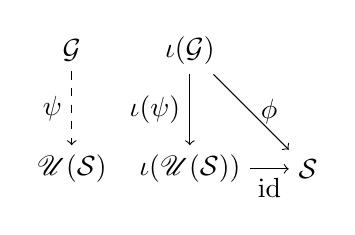
\begin{tikzpicture}
\node (G) at (0,0) {$\mathcal{G}$};
\node (GS) at ([shift={+(0,-1.5)}]G) {$\mathscr{U}(\mathcal{S})$};
\node (iG) at ([shift={+(1.5,0)}]G) {$\iota(\mathcal{G})$};
\node (iGS) at ([shift={+(1.5,-1.5)}]G) {$\iota(\mathscr{U}(\mathcal{S}))$};
\node (S) at ([shift={+(1.5,0)}]iGS) {$\mathcal{S}$};
\draw[->,dashed] (G)--(GS) node[left,midway] {$\psi$};
\draw[->] (iG)--(iGS) node[left,midway] {$\iota(\psi)$};
\draw[->] (iG)--(S) node[right,midway] {$\phi$};
\draw[->] (iGS)--(S) node[below,midway] {$\id$};


\end{tikzpicture}\end{document}